\chapter{Zero density theorems}\label{zero-density-chapter}

\begin{definition}[Zero density exponents]\label{zero-def}  For $\sigma \in \R$ and $T>0$, let $N(\sigma,T)$ denote the number of zeroes $\rho$ of the Riemann zeta function with $\mathrm{Re}(\rho) \geq \sigma$ and $|\mathrm{Im}(\rho)| \leq T$.

If $1/2 \leq \sigma < 1$ is fixed, we define the zero density exponent $\A(\sigma) \in [-\infty,\infty)$ to be the infimum of all (fixed) exponents $A$ for which one has
    $$ N(\sigma-\delta,T) \ll T^{A (1-\sigma)+o(1)}$$
whenever $T$ is unbounded and $\delta>0$ is infinitesimal.
\end{definition}

The shift by $\delta$ is for technical convenience, it allows for $\A(\sigma)$ to control (very slightly) the zeroes to the left of $\mathrm{Re} s = \sigma$.  In non-asymptotic terms: $\A(\sigma)$ is the infimum of all $A$ such that for every $\eps>0$ there exists $C, \delta > 0$ such that
$$ N(\sigma-\delta, T) \leq C T^{A(1-\sigma)+\eps}$$
whenever $T \geq C$.

\begin{lemma}[Basic properties of $A$]\label{zero-basic}\uses{zero-def}
\begin{itemize}
\item[(i)] $\sigma \mapsto (1-\sigma) \A(\sigma)$ is non-increasing and left-continuous, with $\A(1/2)=2$.
\item[(ii)] If the Riemann hypothesis holds, then $\A(\sigma)=-\infty$ for all $1/2 < \sigma \leq 1$.
\end{itemize}
\end{lemma}

\begin{proof} The claim (i) is clear using the Riemann-von Mangoldt formula \cite[Theorem 1.7]{ivic} and the functional equation.  The claim (ii) is also clear.
\end{proof}

\begin{remark} One can ask what happens if one omits the $\delta$ shift.  Thus, define $\A_0(\sigma)$ to be the infimum of all fixed exponents $A$ for which  $N(\sigma,T) \ll T^{A (1-\sigma)+o(1)}$ for unbounded $T$. Then it is not difficult to see that
$$ \lim_{\sigma' \to \sigma^+} \A(\sigma) \leq \A_0(\sigma) \leq \A(\sigma)$$
for any fixed $1/2 < \sigma < 1$; thus $\A_0$ is basically the same exponent at $\A$, except possibly at jump discontinuities of the left-continuous function $\A$, in which case it could theoretically take on a different value.  (But we do not expect such discontinuities to actually exist.)  Thus there is not a major difference between $\A(\sigma)$ and $\A_0(\sigma)$, but the former has some very slight technical advantages (such as the aforementioned left continuity).
\end{remark}

The quantity $\|\A\|_\infty := \sup_{1/2 \leq \sigma < 1} \A(\sigma)$ is of particular importance to the theory of primes in short intervals; see Section \ref{primes-sec}.  From Lemma \ref{zero-basic} we have $\|\A\|_\infty \geq 2$.  It is conjectured that this is an equality.

\begin{conjecture}[Density hypothesis]\label{density-hypothesis}\uses{zero-def}  One has $\|\A\|_\infty=2$.  Equivalently, $\A(\sigma) \leq 2$ for all $1/2 \leq \sigma < 1$.
\end{conjecture}

Indeed, the Riemann hypothesis implies the stronger assertion that $\A(\sigma) = -\infty$ for all $12 < \sigma < 1$.  However, for many applications to the prime numbers in short intervals, the density hypothesis is almost as powerful; see Section \ref{primes-sec}.

Upper bounds on $\A(\sigma)$ can be obtained from large value theorems via the following relation.

\begin{lemma}[Zero density from large values]\label{zero-from-large}\uses{zero-def,lv-def, lvz-def}  Let $1/2 < \sigma < 1$.  Then
$$ \A(\sigma)(1-\sigma) \leq \max( \sup_{\tau \geq 2} \LV_\zeta(\sigma,\tau)/\tau, \limsup_{\tau \to \infty} \LV(\sigma,\tau)/\tau ).$$
\end{lemma}

\begin{proof}\uses{lv-basic}
Write the right-hand side as $B$, then $B \geq 0$ (from Lemma \ref{lv-basic}(iii)) and we have
\begin{equation}\label{lvz-bound}
    \LV_\zeta(\sigma,\tau) \leq B \tau
\end{equation}
for all $\tau \geq 1$, and
\begin{equation}\label{lv-bound}
    \LV(\sigma,\tau) \leq (B+\eps) \tau
\end{equation}
whenever $\eps>0$ and $\tau$ is sufficiently large depending on $\eps$ (and $\sigma$).  It would suffice to show, for any $\eps>0$, that $N(\sigma-o(1),T) \ll T^{B+O(\eps)+o(1)}$ as $T \to \infty$.

By dyadic decomposition, it suffices to show for large $T$ that the number of zeroes with real part at least $\sigma-o(1)$ and imaginary part in  $[T,2T]$ is $\ll T^{B+O(\eps)+o(1)}$.  From the Riemann-von Mangoldt theorem, there are only $O(\log T)$ zeroes whose imaginary part is within $O(1)$ of a specified ordinate $t \in [T,2T]$, so it suffices to show that given some zeroes $\sigma_r + i t_r$, $r=1,\dots,R$ with $\sigma-o(1) \leq \sigma_r < 1$ and $t_r \in [T,2T]$ $1$-separated, that $R \ll T^{B+O(\eps)+o(1)}$.

Suppose that one has a zero $\sigma_r+i t_r$ of this form.  Then by a standard approximation to the zeta function \cite[Theorem 1.8]{ivic}, one has
$$ \sum_{n \leq T} \frac{1}{n^{\sigma_r+it_r}} \ll T^{-1/2}.$$
Let $0 < \delta_1 < \eps$ be a small quantity (independent of $T$) to be chosen later, and let $0 < \delta_2 < \delta_1$ be sufficiently small depending on $\delta_1,\delta_2$.  By the triangle inequality, and refining the sequence $t_r$ by a factor of at most $2$, we either have
$$ \bigg|\sum_{T^{\delta_1} \leq n \leq T} \frac{1}{n^{\sigma_r+it_r}} \bigg| \gg T^{-\delta_2}$$
for all $r$, or
\begin{equation}\label{td}
 \sum_{n \leq T^{\delta_1}} \frac{1}{n^{\sigma_r+it_r}} \ll T^{-\delta_2}
\end{equation}
for all $r$.

Suppose we are in the former (``Type I'') case, we perform a smooth partition of unity, and conclude that
$$ \bigg|\sum_{T^{\delta_1} \leq n \leq T} \frac{\psi(n/N)}{n^{\sigma_r+it_r}} \bigg| \gg T^{-\delta_2 - o(1)}$$
for some fixed bump function $\psi$ supported on $[1/2,1]$, and some $T^{\delta_1} \ll N \ll T$.

We divide into several cases depending on the size of $N$.  First suppose that $N \ll T^{1/2}$.  The variable $n$ is restricted to the interval $I := [\max(N/2, T^{\delta_1}), N]$.  We have
$$ \bigg|\sum_{n \in I} \psi(n/N) (n/N)^{-\sigma_r} n^{-it_r} \bigg| \gg N^\sigma T^{-\delta_2 - o(1)}.$$
Performing a Fourier expansion of $\psi(n/N) (n/N)^{-\sigma_r}$ in $\log n$ and using the triangle inequality, we can bound
$$ \sum_{n \in I} \psi(n/N) (n/N)^{-\sigma_r} n^{-it_r}  \ll_A \int_\R \bigg| \sum_{n \in I} \frac{1}{n^{it}} \bigg| (1+|t-t_r|)^{-A}\ dt$$
for any $A>0$, so by the triangle inequality we conclude that
$$ \bigg|\sum_{n \in I} n^{-it'_r} \bigg| \gg N^\sigma T^{-\delta_2 - o(1)}$$
for some $t'_r = t_r + O(T^{o(1)})$.  By refining the $t_r$ by a factor of $T^{o(1)}$ if necessary, we may assume that the $t'_r$ are $1$-separated, and by passing to a subsequence we may assume that $T = N^{\tau+o(1)}$ for some $2 \leq \tau \leq 1/\delta_1$, then
we conclude that
$$ \bigg| \sum_{n \in I} \frac{1}{n^{it'_r}} \bigg| \gg N^{\sigma-\delta_2/\delta_1+o(1)}$$
for all remaining $r$.  By Definition \ref{lvz-def} we then have (for $\delta_2$ small enough)
$$ R \ll N^{\LV_\zeta(\sigma,\tau) + \eps + o(1)} \ll T^{\LV_\zeta(\sigma,\tau)/\tau + \eps + o(1)}$$
and the claim follows in this case from \eqref{lvz-bound}.

In the case $N \asymp T$, a standard application of the Euler--Maclaurin formula (see e.g., \cite[(2.1.2)]{titchmarsh_theory_1986}) yields
$$ \sum_{T^{\delta_1} \leq n \leq T} \frac{\psi(n/N)}{n^{\sigma_r+it_r}} \ll T^{-\sigma_r}$$
which leads to a contradiction.  So the only remaining case is when $T^{1/2} \ll N \ll o(T)$.  Here we can ignore the cutoffs on $n$ and obtain
$$ \left| \sum_{n} \psi(n/N) (n/N)^{-\sigma_r} n^{-it_r}\right| \gg N^{\sigma} T^{-\delta_2-o(1)}.$$
Applying the van der Corput $B$-process (see, e.g., \cite[\S 8.3]{ik}) or the approximate functional equation we have
$$ \sum_{n} \psi(n/N) (n/N)^{-\sigma_r} n^{-it_r} = e(\frac{t_r}{2\pi} \log \frac{t_r}{2\pi} - \frac{t_r}{2\pi} + \frac{1}{8}) \sum_{m} \psi(2\pi t_r/mN) (2\pi t_r/mN)^{-\sigma_r} m^{it_r} (2\pi m^2/t_r)^{-1/2} + O(T^{o(1)})$$
and thus
$$ \left| \sum_{m} \psi(2\pi t_r/mN) (2\pi t_r/mN)^{1-\sigma_r} m^{-it_r} \right| \gg M^{1/2} N^{\sigma-1/2} T^{-\delta_2-o(1)};$$
where $M := 2\pi T/N \ll N^{1/2}$.  In particular
$$ \sum_{m \in [M/10, 10 M]} \psi(2\pi t_r/mN) (2\pi t_r/mN)^{1-\sigma_r} m^{-it_r} \gg M^{\sigma} T^{-\delta_2-o(1)};$$
since $N \gg T^{1/2}$ and $\sigma \geq 1/2$.  Performing a Fourier expansion as before, we conclude that
$$ \sum_{m \in [M/10, 10 M]} m^{-it'_r} \ll M^{\sigma} T^{-\delta_2-o(1)}$$
for some $t'_r = t_r + O(T^{o(1)})$, and one can argue as in the $N \ll T^{1/2}$ case (partitioning $[M/10, 10M]$ into $O(1)$ intervals each contained in some $[M',2M']$ with $M' \ll T^{1/2}$).

Now suppose instead we are in the latter (``Type II'') case \eqref{td}.  We multiply both sides of \eqref{td} by the mollifier $\sum_{m \leq T^{\delta_2/2}} \frac{1}{m^{\sigma_r+it_r}}$ to obtain
$$ \bigg| 1 + \sum_{T^{\delta_2/2} \leq n \leq T^{\delta_1+\delta_2/2}} \frac{a_n}{n^{\sigma_r+it_r}} \bigg| = o(1)$$
where $a_n$ is some sequence with $a_n \ll T^{o(1)}$.  By dyadic decomposition and the pigeonhole principle, and refining the $t_r$ by a factor of $O(T^{o(1)})$ as needed, we can then find an interval $I$ in $[N,2N]$ with $T^{\delta_2/2} \ll N \ll T^{\delta_1+\delta_2/2}$ such that
$$ \bigg| \sum_{n \in I} \frac{a_n}{n^{\sigma_r+it_r}} \bigg| \gg T^{-o(1)}$$
and hence by Fourier expansion of $\frac{1}{n^{\sigma_r}}$ in $\log n$
$$ \bigg| \sum_{n \in I} \frac{a_n}{n^{it'_r}} \bigg| \gg N^{\sigma_r} T^{-o(1)}$$
for some $t'_r = t_r + O(T^{o(1)})$; by refining the $t_r$ by a further factor of $T^{o(1)}$ we may assume that the $t'_r$ are also $1$-separated; we can also pigeonhole so that $T = N^{\tau+o(1)}$ for some $\frac{1}{\delta_1+\delta_2/2} \leq \tau \leq \frac{1}{\delta_2/2}$.  Applying Lemma \ref{lv-asymp}, we conclude that
$$ R \ll N^{\LV(\sigma,\tau)+o(1)} = T^{\LV(\sigma,\tau)/\tau+o(1)}$$
and the claim follows in this case from \eqref{lv-bound}.
\end{proof}

Recently, a partial converse to the above lemma was established:

\begin{lemma}[Large values from zero density]\label{zero-dens_implies_large}\cite[Theorem 1.2]{matomaki_teravainen_2024}\uses{zero-def, lvz-def} If $\tau > 0$ and $1/2 \leq \sigma \leq 1$ are fixed, then
    $$ \LV_\zeta(\sigma,\tau)/\tau \leq \max\left( \frac{1}{2}, \sup_{\sigma \leq \sigma' \leq 1} \A(\sigma')(1-\sigma') + \frac{\sigma'-\sigma}{2} \right).$$
\end{lemma}

\begin{proof}  Let $N \geq 1$ be unbounded, $T = N^{\tau+o(1)}$, and $I \subset [N,2N]$ be an interval, and $t_1,\dots,t_R \in [T,2T]$ be $1$-separated with
$$ \bigg| \sum_{n \in I} \frac{1}{n^{it_r}} \bigg| \gg N^{\sigma-o(1)}$$
uniformly for all $r$.  By \cite[Theorem 1.2]{matomaki_teravainen_2024}, we have for any fixed $\delta>0$ that
$$ R \ll T^\delta \sup_{\sigma-\delta \leq \sigma' \leq 1} T^{\frac{\sigma' - \sigma}{2}} N(\sigma', O(T)) + T^{\frac{1-\sigma}{2}+\delta}.$$
Using Definition \ref{zero-def}, we conclude that
$$ R \ll T^{\max( \frac{1}{2}, \sup_{\sigma-\delta \leq \sigma' \leq 1} \A(\sigma')(1-\sigma') + \frac{\sigma'-\sigma}{2} ) + O(\delta)}$$
and thus
$$ \LV_\zeta(\sigma,\tau) \leq \tau \max( \frac{1}{2}, \sup_{\sigma-\eps \leq \sigma' \leq 1} \A(\sigma')(1-\sigma') + \frac{\sigma'-\sigma}{2} ) + O(\delta).$$
Here the implied constant in the $O()$ notation is understood to be uniform in $\delta$.
Letting $\delta$ go to zero, and using left-continuity of $\A$, we obtain the claim.
\end{proof}

The suprema in Lemma \ref{zero-from-large} require unbounded values of $\tau$, but thanks to the ability to raise to a power, we can reduce to a bounded range of $\tau$.  Here is a basic such reduction, suited for machine-assisted proofs:

\begin{corollary}\label{zero-large-cor-0} Let $1/2 < \sigma < 1$ and $\tau_0 > 0$.  Then
    $$ \A(\sigma)(1-\sigma) \leq \max \left(\sup_{2 \leq \tau < \tau_0} \LV_\zeta(\sigma,\tau)/\tau, \sup_{\tau_0 \leq \tau \leq 2\tau_0} \LV(\sigma,\tau)/\tau\right)$$
    with the convention that the first supremum is $-\infty$ if it is vacuous (i.e., if $\tau_0 < 2$).
\end{corollary}
\python{zero_density_estimate}
\code{lv_zlv_to_zd(hypotheses, sigma_interval, tau0)}

\begin{proof}
Denote the right-hand side by $B$, thus
    $$ \LV(\sigma,\tau) \leq B\tau$$
    for all $\tau_0 \leq \tau \leq 2\tau_0$, and
    \begin{equation}\label{lvz-b}
         \LV_\zeta(\sigma,\tau) \leq B\tau
    \end{equation}
    whenever $2 \leq \tau < \tau_0$.  From Lemma \ref{power-lemma} we then have
    $$ \LV(\sigma,\tau) \leq B\tau$$
    for all $k\tau_0 \leq \tau \leq 2k\tau_0$ and natural numbers $k$. Note that the intervals $[k\tau_0, 2k\tau_0]$ cover all of $[\tau_0,\infty)$, hence we have
    $$ \LV(\sigma,\tau) \leq B\tau$$
    for all $\tau \geq \tau_0$. In particular
    $$ \limsup_{\tau \to \infty} \LV(\sigma,\tau)/\tau  \leq B.$$
    Also, combining the previous estimate with \eqref{lvz-b} using Lemma \ref{lvz-basic}(iii) we have
    \begin{equation}\label{lvzo}
     \LV_\zeta(\sigma,\tau) \leq B\tau
    \end{equation}
    for all $\tau \geq 2$.  By Lemma \ref{lvz-basic}(iv), this implies that
    $$ \LV_\zeta\bigg(\frac{1}{2} + \frac{1}{\tau-1} (\sigma-\frac{1}{2}), \frac{\tau}{\tau-1} \bigg) \leq B \frac{\tau}{\tau-1}$$
    for $\tau \geq 2$.  Thus
    $$ \sup_{\tau \geq 2} \frac{\LV_\zeta(\sigma,\tau)}{\tau} \leq B.$$
    The claim now follows from Lemma \ref{zero-from-large}.
\end{proof}

For machine assisted proofs, one can simply take $\tau_0$ to be a sufficiently large quantity, e.g., $\tau_0=3$ for $\sigma$ not too close to $1$, and larger for $\sigma$ approaching $1$, to recover the full power of Lemma \ref{zero-from-large}.  However, the amount of case analysis required increases with $\tau_0$.  For human written proofs, the following version of Corollary \ref{zero-large-cor-0} is more convenient:

\begin{corollary}\label{zero-large-cor} Let $1/2 < \sigma < 1$ and $\tau_0 > 0$.  Then
$$ \A(\sigma)(1-\sigma) \leq \max \left(\sup_{2 \leq \tau < 4\tau_0/3} \LV_\zeta(\sigma,\tau)/\tau, \sup_{2\tau_0/3 \leq \tau \leq \tau_0} \LV(\sigma,\tau)/\tau\right).$$
\end{corollary}

\python{zero_density_estimate}
\code{lv_zlv_to_zd2(hypotheses, sigma_interval, tau0)}

\begin{proof}\uses{zero-large-cor-0, power-lemma}  Applying Corollary \ref{zero-large-cor-0} with $\tau$ replaced by $4\tau_0/3$, it suffices to show that
$$\sup_{4\tau_0/3 \leq \tau \leq 8\tau_0/3} \LV(\sigma,\tau)/\tau \leq \sup_{2\tau_0/3 \leq \tau \leq \tau_0} \LV(\sigma,\tau)/\tau.$$
But this follows from Lemma \ref{power-lemma}, since the intervals $[2k\tau_0/3, k\tau_0]$ for $k=2,3$ cover all of $[4\tau_0/3,8\tau_0/3]$.
\end{proof}

The following special case of the above corollary is frequently used in practice to assist with the human readability of zero density proofs:

\begin{corollary}\label{zero-large-cor2}\uses{zero-def, lvz-def, lv-def, zero-large-cor} Let $1/2 < \sigma < 1$ and $\tau_0 > 0$.  Suppose that one has the bounds
\begin{equation}\label{lvo}
\LV(\sigma,\tau) \leq (3-3\sigma) \frac{\tau}{\tau_0}
\end{equation}
for $2\tau_0/3 \leq \tau \leq \tau_0$, and
\begin{equation}\label{lvoz}
 \LV_\zeta(\sigma,\tau) \leq (3-3\sigma) \frac{\tau}{\tau_0}
\end{equation}
for $2 \leq \tau < 4\tau_0/3$.  Then $\A(\sigma) \leq \frac{3}{\tau_0}$.
\end{corollary}

The reason why this particular special case is convenient is because the inequality
\begin{equation}\label{obvious}
    2 - 2\sigma \leq (3-3\sigma) \frac{\tau}{\tau_0}
\end{equation}
obviously holds for $\tau \geq 2\tau_0/3$.  That is to say, we automatically verify \eqref{lvo} in regimes where the Montgomery conjecture holds. In fact, we can do a bit better, thanks to subdivision:

\begin{corollary}\label{zero-large-cor3}\uses{zero-def, lv-def} Let $1/2 < \sigma < 1$ and $\tau_0 > 0$. Suppose that one has the bound \eqref{lvoz}
   for $2 \leq \tau < 4\tau_0/3$, and the Montgomery conjecture $\LV(\sigma,\tau) \leq 2-2\sigma$ whenever $0 \leq \tau \leq \tau_0+\sigma-1$.  Then $\A(\sigma) \leq \frac{3}{\tau_0}$.
\end{corollary}

\begin{proof}\uses{lv-basic, zero-large-cor2}  We may assume that $\tau_0 \geq 3-3\sigma$, since otherwise the claim follows from the Riemann--von Mangoldt bound
    $$ \A(\sigma)(1-\sigma) \leq \A(1/2)(1-1/2) = 1.$$
    By Lemma \ref{lv-basic}(ii) we have
$$ \LV(\sigma,\tau) \leq \max( 2-2\sigma, 3-3\sigma + \tau - \tau_0 )$$
for all $\tau \geq 0$.  But both expressions on the right-hand side are bounded by $(3-3\sigma) \frac{\tau}{\tau_0}$ for $2\tau_3 \leq \tau \leq \tau_0$ and $\tau_0 \geq 3-3\sigma$, so the claim follows from Corollary \ref{zero-large-cor2}.
\end{proof}

\section{Known zero density bounds}

Let us see some examples of these corollaries in action.

\begin{theorem}\label{montgomery_implies_density}\uses{density-hypothesis} The Montgomery conjecture implies the density hypothesis.
\end{theorem}

\begin{proof}\uses{zero-large-cor2}  Apply Corollary \ref{zero-large-cor2} with $\tau_0=3/2$ (so that \eqref{lvoz} is vacuously true).
\end{proof}

\begin{theorem}\label{lindelof_implies_density}\uses{density-hypothesis} The Lindelof hypothesis implies the density hypothesis, and also that $\A(\sigma) \leq 0$ for $3/4 < \sigma \leq 1$.
\end{theorem}

\begin{proof}\uses{zero-large-cor, lh-vanish, l2-mvt, power-lemma, htlv} The first result is proved in \cite{ingham_estimation_1940}, and the second result is due to \cite{halasz_distribution_1969}. We will apply Corollary \ref{zero-large-cor}.  From Corollary \ref{lh-vanish} we see that $\LV_\zeta(\sigma,\tau) = -\infty$ whenever $\sigma > 1/2$ and $\tau \geq 1$, so for any choice of $\tau_0$ we have
$$ \sup_{2 \leq \tau < 4\tau_0/3} \LV_\zeta(\sigma,\tau)/\tau = -\infty.$$
From Theorem \ref{l2-mvt} and Lemma \ref{power-lemma} we have
\begin{equation}\label{ap}
     \LV(\sigma,\tau) \leq \max( (2-2\sigma)k, \tau + (1 - 2 \sigma)k )
\end{equation}
for any natural number $k$ and $\tau \geq 1$; setting $k$ to be the integer part of $\tau$ we conclude in particular that
$$ \LV(\sigma,\tau) \leq (2-2\sigma)\tau + O(1),$$
and hence by taking $\tau_0$ large enough, we can make
$\sup_{2\tau_0/3 \leq \tau \leq \tau_0} \LV(\sigma,\tau)/\tau$ bounded by $2-2\sigma + \eps$ for any $\eps>0$.  This already gives the density hypothesis bound $\A(\sigma) \leq 2$.  For $\sigma > 3/4$, we may additionally apply Theorem \ref{htlv} to make
$\sup_{2\tau_0/3 \leq \tau \leq \tau_0} \LV(\sigma,\tau)/\tau$ arbitrarily small, giving the bound $\A(\sigma) \leq 0$.
\end{proof}

There are similar results assuming weaker versions of the Lindelof hypothesis. For instance, we have

\begin{theorem}[Ingham's first bound]\label{thm:ingham-first}\uses{zeta-grow-def, zero-def} \cite{ingham_difference_1937} (See also \cite{titchmarsh_theory_1986}) For any $1/2 < \sigma < 1$, we have
    $$ \A(\sigma) \leq 2 + 4 \mu(1/2).$$
\end{theorem}

\begin{proof}\uses{zero-large-cor-0, lvz-mu} We give here a proof (somewhat different from the original proof) that passes through Corollary \ref{zero-large-cor-0}.
We apply Corollary \ref{zero-large-cor-0} with $\tau_0$ chosen so that $\mu(1/2) \tau_0 < \sigma-1/2$. From Corollary \ref{lvz-mu} we then have
$$ \A(\sigma)(1-\sigma) \leq \sup_{\tau_0 \leq \tau \leq 2\tau_0} \LV(\sigma,\tau)/\tau.$$
For any integer $k \geq 0$ and $k \leq \tau \leq k+1$, we see from \eqref{ap} that
$$ \LV(\sigma,\tau) \leq (2-2\sigma)(k+1)$$
and
$$ \LV(\sigma,\tau) \leq \tau + (1-2\sigma)k;$$
multiplying the first inequality by $2\sigma-1$, the second by $2-2\sigma$, and summing, we conclude that
$$ \LV(\sigma,\tau) \leq (\tau + 2\sigma-1) (2-2\sigma);$$
inserting this bound we have
$$ \A(\sigma) \leq 2 + \frac{2\sigma-1}{\tau_0}.$$
Optimizing in $\tau_0$, we obtain the claim.
\end{proof}

\begin{theorem}[Ingham's second bound]\label{thm:ingham_zero_density2}\cite{ingham_estimation_1940}\uses{zero-def} For any $1/2 < \sigma < 1$, one has $\A(\sigma) \leq \frac{3}{2-\sigma}$.
\end{theorem}
\literature
\code{add_zero_density_ingham_1940()}
\derived
\code{prove_zero_density_ingham_1940()}
\code{prove_zero_density_ingham_1940_v2()}

\begin{proof}\uses{zero-large-cor3, l2-mvt}
We apply Corollary \ref{zero-large-cor3} with $\tau_0 := 2-\sigma$.  Here we have $4\tau_0/3 < 2$ since $\sigma>1/2$, so the claim \eqref{lvoz} is automatic; and the Montgomery conjecture hypothesis follows from Theorem \ref{l2-mvt}.
\end{proof}

Either of Theorem \ref{thm:ingham-first} or Theorem \ref{thm:ingham_zero_density2} implies an older result of Carlson \cite{carlson_uber_1921} that $\A(\sigma) \le 4\sigma$ for $1/2 < \sigma < 1$.
\literature
\code{add_zero_density_carlson_1921()}

\begin{theorem}[Huxley bound]\label{huxley-bound}\cite{Huxley}\uses{zero-def} For any $1/2 < \sigma < 1$, one has $\A(\sigma) \leq \frac{3}{3\sigma-1}$. (In particular, the density hypothesis holds for $\sigma \geq 5/6$.)
\end{theorem}
\literature
\code{add_zero_density_huxley_1972()}
\derived
\code{prove_zero_density_huxley_1972()}
\code{prove_zero_density_huxley_1972_v2()}

\begin{proof}\uses{zero-large-cor3, huxley-lv, lvz-mu} We apply Corollary \ref{zero-large-cor3} with $\tau_0 := 3\sigma-1$.  The Montgomery conjecture hypothesis follows from Theorem \ref{huxley-lv}. So it remains to show that \eqref{lvoz} holds for $2 \leq \tau < 4\tau_0/3$.  For $\sigma \leq 5/6$ we have $4\tau_0/3 \leq 2$, so the claim is vacuously true in this case.  For $\sigma > 5/6$ we use Corollary \ref{lvz-mu} and the bound $\mu(1/2) \leq 1/6$ from Table \ref{mu-table} to conclude that
$\LV_\zeta(\sigma,\tau) = -\infty$ whenever $\sigma > 1/2 + \tau/6$, but this is precisely $\tau < 6\sigma - 3$.  Since $6\sigma-3 > 4\tau_0/3$ when $\sigma > 5/6$, we obtain the claim.
\end{proof}

\begin{theorem}[Guth--Maynard bound]\label{guth-maynard-density}\uses{zero-def}  For any $1/2 < \sigma < 1$, one has $\A(\sigma) \leq \frac{15}{3+5\sigma}$.
\end{theorem}
\literature
\code{add_zero_density_guth_maynard_2024()}
\derived
\code{prove_zero_density_guth_maynard_2024()}
\code{prove_zero_density_guth_maynard_2024_v2()}

\begin{proof}\uses{thm:ingham_zero_density2, huxley-lv,zero-large-cor2, guth-maynard-lvt, l2-mvt} We may assume that $7/10 < \sigma < 8/10$, since the bound follows from the Ingham and Huxley bounds otherwise.  We apply Corollary \ref{zero-large-cor2} with $\tau_0 := \frac{3+5\sigma}{5}$.  We have $4\tau_0/3 < 2$, so the claim \eqref{lvoz} is vacuous and we only need to establish \eqref{lvo}.  We split into the subranges $13/5-2\sigma \leq \tau < \tau_0$ and $2\tau_0/3 \leq \tau \leq 13/5-2\sigma$. In the former range we use Theorem \ref{guth-maynard-lvt} (and \eqref{obvious}), and reduce to showing that
$$ 18/5 - 4 \sigma \leq (3-3\sigma) \frac{\tau}{\tau_0},$$
and
$$ \tau + 12/5 - 4\sigma \leq (3-3\sigma) \frac{\tau}{\tau_0}$$
for $13/5-2\sigma \leq \tau < \tau_0$.  The first inequality follows from
\begin{equation}\label{18-5}
 18/5 - 4 \sigma \leq (3-3\sigma) \frac{13/5-2\sigma}{\tau_0}
\end{equation}
which one can numerically check holds in the range $7/10 < \sigma < 8/10$.  Finally, the third inequality is obeyed with equality when $\tau=\tau_0$ and the right-hand side has a larger slope in $\tau$ than the left (since $\tau_0 \geq 3-3\sigma$), so the claim follows as well.

In the remaining region $2\tau_0/3 \leq \tau \leq 13/5-2\sigma$, we use Theorem \ref{l2-mvt} and \eqref{obvious} to reduce to showing that
$$ \tau + 1 - 2\sigma \leq (3-3\sigma) \frac{\tau}{\tau_0}$$
in this range.  This follows again from \eqref{18-5} which guarantees the inequality at the right endpoint $\tau = 13/5-2\sigma$.
\end{proof}

\begin{theorem}[Jutila zero density theorem]\label{jutila-density} \cite{jutila_zero_density_1977}\uses{density-hypothesis} The zero density hypothesis is true for $\sigma \geq 11/14$.
\end{theorem}
\derived
\code{prove_zero_density_jutila_1977()}
\code{prove_zero_density_jutila_1977_v2()}

\begin{proof}\uses{zero-large-cor, jutila-lvt}
We apply Corollary \ref{zero-large-cor} with $\tau_0 := 3/2$, then it suffices to show that
    $$\LV(\sigma,\tau) \leq (2-2\sigma) \tau$$
    for all $1 \leq \tau \leq 3/2$.

    From the $k=3$ case of Theorem \ref{jutila-lvt} we have
    $$\LV(\sigma,\tau) \leq \max \bigg(2-2\sigma, \tau + \frac{10-16\sigma}{3}, \tau + 18-24\sigma \bigg).$$
    But all terms on the right-hand side can be verified to be less than or equal to $(2-2\sigma)\tau$ when $1 \leq \tau \leq 3/2$ and $\sigma \geq 11/14$, giving the claim.
\end{proof}

In fact, we can do better:

\begin{theorem}[Heath-Brown zero density theorem]\label{hb-density} \cite{heathbrown_zero_1979}\uses{zero-def} For $11/14 \leq \sigma < 1$, one has $\A(\sigma) \leq \frac{9}{7\sigma - 1}$ (in particular, this recovers Theorem \ref{jutila-density}).  For any $3/4 \leq \sigma \leq 1$, one has $\A(\sigma) \leq \max(\frac{3}{10\sigma-7}, \frac{4}{4\sigma-1})$ (which is a superior bound when $\sigma \geq 20/23$).
\end{theorem}
\literature
\code{add_zero_density_heathbrown_1979()}
\derived
\code{prove_zero_density_heathbrown_1979a()}
\code{prove_zero_density_heathbrown_1979b()}
\code{prove_zero_density_heathbrown_1979a_v2()}
\code{prove_zero_density_heathbrown_1979b_v2()}

\begin{proof}\uses{zero-large-cor2, jutila-lvt, hb-12, hb-opt} For the first estimate, we apply Corollary \ref{zero-large-cor2} with $\tau_0 := \frac{7\sigma-1}{3}$.  To verify \eqref{lvo}, we apply the $k=3$ version of Theorem \ref{jutila-lvt}, which gives
$$ \LV(\sigma,\tau) \leq \max \bigg( 2-2\sigma, \tau + \frac{10-16\sigma}{3}, \tau + 18-24\sigma \bigg).$$
When $\sigma \geq 11/14$ one has $18-24\sigma \leq \frac{10-16\sigma}{3}$, so by \eqref{obvious} we need to show that
$$ \tau + \frac{10-16\sigma}{3} \leq (3-3\sigma) \frac{\tau}{\tau_0}$$
for $2\tau_0/3 \leq \tau \leq \tau_0$.  This holds with equality at $\tau=\tau_0$, hence holds for $\tau \leq \tau_0$ as well since $\tau_0 \geq 3-3\sigma$.  As for \eqref{lvoz}, we invoke Theorem \ref{hb-12} and reduce to showing that
$$ 2\tau + 6 - 12\sigma \leq (3-3\sigma) \frac{\tau}{\tau_0}$$
for $2 \leq \tau \leq 4\tau_0/3$.  Since $6-12\sigma$ is negative, the ratio of the left-hand side and right-hand side is increasing in $\tau$, so it suffices to verify this claim at the endpoint $\tau = 4\tau_0/3$.  The claim then simplifies to $\tau_0 \leq \frac{3}{4} (4\sigma-1)$, which one can verify from the choice of $\tau_0$ and the hypothesis $\sigma \geq 11/14$.

For the second estimate, we take $\tau_0 := \min( 10\sigma-7, \frac{3}{4} (4\sigma-1))$.  To verify \eqref{lvo}, we now use Theorem \ref{hb-opt} and \eqref{obvious}, and reduce to showing that
$$ \tau + 10-13\sigma \leq (3-3\sigma) \frac{\tau}{\tau_0}$$
for $2\tau_0/3 \leq \tau \leq \tau_0$.  The inequality holds at $\tau=\tau_0$ since $\tau_0 \leq 10\sigma-7$, and hence for all smaller $\tau$ since $\tau_0 \geq 3-3\sigma$.  As for \eqref{lvoz}, we can repeat the previous arguments since $\tau_0 \leq \frac{3}{4} (4\sigma-1)$.
\end{proof}

With the aid of computer assistance, we were able to strengthen the second claim here.  We first need a lemma:

\begin{lemma}\label{3-40}\uses{exp-pair-def, zeta-grow-def} $(3/40, 31/40)$ is an exponent pair.  In particular, by Corollary \ref{exp-pair-mu}, $\mu(7/10) \leq 3/40$.
\end{lemma}

\derived
\code{best_proof_of_exponent_pair(frac(3,40), frac(31,40))}

\begin{proof}\uses{line-sym, exp-pair-closed, vdc-a, vdc-b, beta-duality, huxley-table, vdc-opt}  This can be derived from the Watt exponent pair $W := (89/560, 1/2 + 89/560)$ from Theorem \ref{line-sym} as well as the $A$ and $B$ transforms and convexity (Lemmas \ref{exp-pair-closed}, \ref{vdc-a}, \ref{vdc-b}) after observing that
$$(3/40,31/40) = xy AW + (1-x)y ABA W + (1-y) W$$
with $x=37081/40415$ and $y=476897/493711$.  (One could of course also use more recent exponent pairs that are stronger, such as the Bourgain exponent pair $(13/84, 1/2+13/84)$.)  We remark that one could also obtain this result from Lemma \ref{beta-duality}, after observing that the required bound $\beta(\alpha) \leq 3/40 + 7\alpha/10$ can be derived from Theorem \ref{huxley-table} (as well as the classical bounds in Corollary \ref{vdc-opt}).  We also note that the corollary $\mu(7/10) \leq 3/40 = 0.075$ is immediate from \cite[Theorem 2.4]{trudgian-yang}, which in fact gives the slightly stronger bound $\mu(7/10) \leq 218/3005 = 0.07254\dots$.
\end{proof}

\begin{theorem}[Improved Heath-Brown zero density theorem]\label{hb-density2}\uses{zero-def} For any $7/10 < \sigma \leq 1$, one has $\A(\sigma) \leq \frac{3}{10\sigma-7}$.
\end{theorem}
\derived
\code{prove_zero_density_heathbrown_extended()}

\begin{proof}\uses{zero-large-cor3, 3-40, hb-opt, lvz-exp}  We apply Corollary \ref{zero-large-cor3} with $\tau_0 := 10\sigma-7$.  The claim \eqref{lvo} again follows from
    Theorem \ref{hb-opt} and \eqref{obvious} as in the proof of Theorem \ref{hb-density}.  Meanwhile, from Lemma \ref{3-40} and Corollary \ref{lvz-exp} we have $\LV_\zeta(\sigma,\tau) = -\infty$ whenever $\sigma > \frac{3}{40} \tau + \frac{7}{10}$, or equivalently $\tau < \frac{4}{3} (10\sigma-7)$, which then immediately gives \eqref{lvoz}.
\end{proof}

\begin{theorem}[Bourgain result on density hypothesis]\label{bourgain-density}\uses{density-hypothesis} The density hypothesis holds for $\sigma > 25/32$.
\end{theorem}

\literature
\code{add_zero_density_bourgain_2000()}

\begin{proof}  The arguments below are a translation of the original arguments of Bourgain \cite{bourgain_large_2000} to our notational framework.

In view of Theorem \ref{jutila-density} (or Theorem \ref{hb-density}), we may assume that $25/32 < \sigma < 11/14$.  Set $\rho := \LV(\sigma,\tau)$. As in the proof of Theorem \ref{jutila-density}, it suffices to show that
\begin{equation}\label{rot}
    \rho \leq (2-2\sigma) \tau
\end{equation}
for all $1 \leq \tau \leq 3/2$.

From the $k=3$ case of Theorem \ref{jutila-lvt} we have
\begin{equation}\label{rhomax}
    \rho \leq \max \bigg(2-2\sigma, \tau + \frac{10-16\sigma}{3}, \tau + 18-24\sigma \bigg)
\end{equation}
which in the $\sigma < 11/14$ regime simplifies to
\begin{equation}\label{r0-start}
\rho \leq \max(2-2\sigma, \tau + 18-24\sigma)
\end{equation}
and this already suffices unless
\begin{equation}\label{tau-check}
     \tau \geq \frac{24\sigma-18}{2\sigma-1}.
\end{equation}
In the regime $\sigma > 25/32$ and $\tau \leq 3/2$, the bound \eqref{r0-start} certainly implies
$$ \rho \leq \min(1, 4-2\tau)$$
and also
$$ \max(1,2\tau-2) = 1$$
so we may invoke Corollary \ref{borg-lv-simp} to conclude that
\begin{equation}\label{40}
     \rho \leq \max( \alpha_2 + 2 - 2 \sigma, \alpha_1+\alpha_2/2 + 2-2\sigma, -\alpha_2 + 2\tau+4-8\sigma, -2\alpha_1 + \tau + 12 - 16 \sigma, 4\alpha_1 + 3-4\sigma)
\end{equation}
for any $\alpha_1, \alpha_2 \geq 0$.

We now divide into cases.  First suppose that $\tau \leq \frac{4(1+\sigma)}{5}$.  In this case we set $\alpha_1 := \frac{\tau}{3} - \frac{2}{3} (7\sigma-5)$ (which can be checked to be nonnegative using \eqref{tau-check} and $\sigma \geq 25/32$) and $\alpha_2=0$, and one can check that \eqref{40} implies \eqref{rot} in this case (with some room to spare).

Now suppose that $\tau > \frac{4(1+\sigma)}{5}$.  In this case we choose $\alpha_1 = \frac{\tau}{8} - \frac{9\sigma-7}{2}$ and $\alpha_2 = \frac{5\tau}{4} - (1+\sigma)$, which can be checked to be nonnegative using the hypotheses on $\sigma,\tau$.  In this case
one can again check that \eqref{40} implies \eqref{rot}.
\end{proof}

We can improve this bound as follows:

\begin{theorem}[Improved Bourgain density hypothesis bound]\label{bourgain-density-improved}\uses{zero-def} For $17/22 \leq \sigma \leq 4/5$, one has $\A(\sigma) \leq \max( \frac{2}{9\sigma-6}, \frac{9}{8(2\sigma-1)} )$.  Thus one has $\A(\sigma) \leq \frac{9}{8(2\sigma-1)}$ for $38/49 \leq \sigma \leq 4/5$ and $\A(\sigma) \leq \frac{2}{9\sigma-6}$ for $17/22 \leq \sigma \leq 38/49$.
\end{theorem}
\derived
\code{prove_zero_density_bourgain_improved()}

The arguments can be pushed to some $\sigma$ below $17/22$, but in that range the estimate in Corollary \ref{further_ivic_zero} becomes superior, so we do not pursue this further.

\begin{proof}\uses{zero-large-cor3, hb-12, jutila-lvt, borg-lv-simp}  We apply Corollary \ref{zero-large-cor3} with $\tau_0 := \min( \frac{ 9(3\sigma-2)}{2}, \frac{8(2\sigma-1)}{3} )$.  For future reference we note that
\begin{equation}\label{slope}
    \frac{1}{3} < \frac{3-3\sigma}{\tau_0} < \frac{1}{2}.
\end{equation}

It suffices to show that
\begin{equation}\label{lv-st}
 \LV(\sigma,\tau) \leq \frac{\tau}{\tau_0} (3-3\sigma)
\end{equation}
for $2\tau_0/3 \leq \tau \leq \tau_0$, as well as
\begin{equation}\label{lvz-st}
\LV_\zeta(\sigma,\tau) \leq \frac{\tau}{\tau_0} (3-3\sigma)
\end{equation}
for $2 \leq \tau < 4\tau_0/3$.
For \eqref{lvz-st} we use the twelfth moment bound in Theorem \ref{hb-12}.  Since the slope of
$2\tau - 12 (\sigma-1/2)$ in $\tau$ exceeds that of $\frac{\tau}{\tau_0} (3-3\sigma)$ by \eqref{slope}, it suffices to check the bound at the endpoint, i.e., to show that
$$ 8\tau_0/3 - 12 (\sigma-1/2) \leq 4 -4\sigma$$
or equivalently $\tau_0 \leq \frac{3(4\sigma-1)}{4}$, which one can easily check to be the case.

Now we prove \eqref{lv-st}.  Set $\rho := \LV(\sigma,\tau)$.  From the $k=3$ case of Theorem \ref{jutila-lvt} we again have
\eqref{rhomax}, which implies the required bound $\rho \leq \frac{\tau}{\tau_0}(3-3\sigma)$ unless one has
\begin{equation}\label{tau-lower}
    \tau \geq - \max( \frac{10-16\sigma}{3}, 18-24\sigma) / (1 - \frac{3-3\sigma}{\tau_0})
\end{equation}
In this regime, one can also check from \eqref{rhomax} that
$$ \rho \leq \min(1, 4-2\tau)$$
(with room to spare) so we may apply Corollary \ref{borg-lv-simp} to obtain
\begin{equation}\label{40-alt}
\begin{split}
\rho &\leq \max( \alpha_2 + 2 - 2 \sigma, \alpha_1+\alpha_2/2 + 2-2\sigma, -\alpha_2 + 2\tau+4-8\sigma, \\
&\qquad\qquad -2\alpha_1 + \tau + 12 - 16 \sigma, 4\alpha_1 + 2+\max(1,2\tau-2)-4\sigma)
\end{split}
\end{equation}
for any $\alpha_1, \alpha_2 \geq 0$.

We first consider the case when $38/49 \leq \sigma \leq 4/5$, so that $\tau_0 = 8(2\sigma-1)/3$.
As in the proof of Theorem \ref{bourgain-density}, we set
$$ \alpha_2 := \max\left( \frac{5\tau}{4} - (1+\sigma), 0\right)$$
and
$$ \alpha_1 := \frac{\tau}{3} - \frac{2}{3} (7\sigma-5) - \alpha_2/6.$$
With this choice, the expressions $\alpha_1+\alpha_2/2 + 2-2\sigma$ and $-2\alpha_1 + \tau + 12 - 16 \sigma$ are both equal to
$\frac{\tau}{3} + \frac{16-20\sigma}{3} + \frac{\alpha_2}{3}$, while $-\alpha_2 + 2\tau+4-8\sigma$ is equal to
$$ \frac{\tau}{3} + \frac{16-20\sigma}{3} + \frac{\alpha_2}{3} - \frac{4}{3} \left(\alpha_2 - \frac{5\tau}{4} - (1+\sigma)\right)$$
which is less than or equal to the previous expression by definition of $\alpha_2$.  Finally, the expression
$4\alpha_1 + 1+\max(2,2\tau-2)-4\sigma$ is equal to
$$ \frac{4\tau}{3} + \frac{46-68\sigma}{3} + \max(1,2\tau-2) - \frac{2\alpha_2}{3}.$$
Thus it remains to show the bounds
\begin{equation}\label{bound-1}
 \alpha_2 + 2 - 2 \sigma \leq \frac{\tau}{\tau_0} (3-3\sigma)
\end{equation}
\begin{equation}\label{taut}
    \frac{\tau}{3} + \frac{16-20\sigma}{3} + \frac{\alpha_2}{3} \leq \frac{\tau}{\tau_0} (3-3\sigma)
\end{equation}
and
\begin{equation}\label{tar}
    \frac{4\tau}{3} + \frac{46-68\sigma}{3}+ \max(1,2\tau-2) - \frac{2\alpha_2}{3} \leq \frac{\tau}{\tau_0} (3-3\sigma).
\end{equation}
For \eqref{bound-1}, we trivially have $2-2\sigma \leq \frac{\tau}{\tau_0}(3-3\sigma)$ since $\tau \geq 2\tau_0/3$, and the slope of $\frac{5\tau}{4} - (1+\sigma) + 2-2\sigma$ in $\tau$ certainly exceeds $\frac{3-3\sigma}{\tau_0}$ by \eqref{slope}, so it suffices to check the endpoint
$$ \frac{5\tau_0}{4} - (1+\sigma) + 2-2\sigma \leq 3-3\sigma$$
which one can check to be valid for $\sigma \leq 4/5$. Now we turn to \eqref{taut}.  From \eqref{slope} it suffices to show that
$$ \frac{\tau_0}{3} + \frac{16-20\sigma}{3} + \frac{\frac{5\tau_0}{4} - (1+\sigma)}{3} \leq 3 -3 \sigma$$
and
$$ \frac{\tau}{3} + \frac{16-20\sigma}{3} + \frac{0}{3} \leq 2 -2 \sigma.$$
The former is an identity, and the latter simplifies to $\tau \geq 14\sigma-10$, which one can check follows from \eqref{tau-lower} (with some room to spare) in the regime $38/49 \leq \sigma \leq 4/5$, giving the claim.  Finally, for \eqref{tar} it suffices to show that
$$ \frac{4\tau}{3} + \frac{46-68\sigma}{3}  + \max(1,2\tau_0-2) - \frac{2(\frac{5\tau}{4} - (1+\sigma))}{3} \leq \frac{\tau}{\tau_0} (3-3\sigma)$$
which by \eqref{slope} would follow from
$$ \frac{4\tau_0}{3} + \frac{46-68\sigma}{3} + \max(1,2\tau_0-2) - \frac{2(\frac{5\tau_0}{4} - (1+\sigma))}{3} \leq 3-3\sigma$$
and one can check that this applies for $\sigma \geq 38/49$.

Now suppose that we are in the case $17/22 \leq \sigma \leq 38/49$, so that $\tau_0 = \frac{9(3\sigma-2)}{2} \leq \frac{72}{49} < \frac{3}{2}$ (so in particular $\max(1,2\tau-2) = 1$ for $\tau \leq \tau_0$).  We set
$$ \alpha_2 := \max(11 - 16 \sigma + \tau,0)$$
and
$$ \alpha_1 := \frac{\tau}{3} - \frac{2}{3} (7\sigma-5) - \alpha_2/6.$$
Note that for $\sigma \leq 38/49$, one has
$$ (5\tau/4 - (1+\sigma)) - (11 - 16 \sigma + \tau) \leq 15\sigma - 12 - \tau_0/4 \leq 0$$
and hence
$$ \alpha_2 \geq 5\tau/4 - (1+\sigma).$$
As before, we conclude that the quantities $\alpha_1+\alpha_2/2 + 2-2\sigma$ and $-2\alpha_1 + \tau + 12 - 16 \sigma$ are both equal to $\frac{\tau}{3} + \frac{16-20\sigma}{3} + \frac{\alpha_2}{3}$, while $-\alpha_2 + 2\tau+4-8\sigma$ is less than or equal to this quantity.  Thus it suffices to show \eqref{bound-1}, \eqref{taut}, \eqref{tar} as before.

For \eqref{bound-1} we argue as before to reduce to showing that
$$ 11 - 16 \sigma + \tau_0 + 2 - 2 \sigma \leq 3 - 3\sigma$$
which one can check to be true (with room to spare) for $\sigma \geq 17/22$.  For \eqref{taut}, we use \eqref{slope} as before to reduce to showing that
$$ \frac{\tau_0}{3} + \frac{16-20\sigma}{3} + \frac{11 - 16 \sigma + \tau}{3} \leq 3 -3 \sigma$$
and
$$ \frac{\tau}{3} + \frac{16-20\sigma}{3} + \frac{0}{3} \leq 2 -2 \sigma.$$
The first inequality is an identity, and the latter again reduces to  $\tau \geq 14\sigma-10$ which one can check follows from \eqref{tau-lower}.  For \eqref{tar} it suffices to show that
$$ \frac{4\tau}{3} + \frac{46-68\sigma}{3}  + 1 - \frac{2(11 - 16 \sigma + \tau)}{3} \leq \frac{\tau}{\tau_0} (3-3\sigma)$$
which by \eqref{slope} follows from
$$ \frac{4\tau_0}{3} + \frac{46-68\sigma}{3}  + 1 - \frac{2(11 - 16 \sigma + \tau_0)}{3} \leq 3 - 3\sigma,$$
but this is an identity.
\end{proof}

\begin{theorem}[Bourgain zero density theorem]\label{bourgain-zd}\cite[Proposition 3]{bourgain_remarks_1995}\uses{exp-pair-def, zero-def}  Let $(k,\ell)$ be an exponent pair with $k < 1/5$, $\ell > 3/5$, and $15\ell + 20k > 13$.  Then, for any $\sigma > \frac{\ell+1}{2(k+1)}$, one has
    $$ \A(\sigma) \leq \frac{4k}{2(1+k)\sigma - 1 - \ell}$$
    assuming either that $k < \frac{11}{85}$, or that $\frac{11}{85} < k < \frac{1}{5}$ and $\sigma > \frac{144k-11\ell-11}{170k-22}$.
\end{theorem}

\begin{corollary}[Special case of Bourgain's zero density theorem]\label{bourgain-zero-density}\cite[Corollary 4]{bourgain_remarks_1995}\uses{zero-def}  One has
    $$ \A(\sigma) \leq \frac{4}{30\sigma-25}$$
    for $\frac{15}{16} \leq \sigma \leq 1$
    and
    $$ \A(\sigma) \leq \frac{2}{7\sigma-5}$$
    for $\frac{17}{19} \leq \sigma \leq \frac{15}{16}$.
\end{corollary}

\literature
\code{add_zero_density_bourgain_1995()}

\begin{proof}\uses{bourgain-zd, vdc-class} Apply Theorem \ref{bourgain-zd} with the classical pairs $(\frac{1}{14},\frac{11}{14})$ and $(\frac{1}{6}, \frac{2}{3})$ respectively from Proposition \ref{vdc-class}.
\end{proof}

It was remarked in \cite{bourgain_remarks_1995} that further zero density estimates could be obtained by using additional exponent pairs.  This we do here:

\begin{corollary}[Optimized Bourgain zero density bound]\label{bourgain-zero-density-optimized}\uses{zero-def} One has
\[
\A(\sigma) \leq \begin{cases}
\dfrac{11}{12(4 \sigma - 3)} & \dfrac{3}{4} < \sigma \le \dfrac{14}{15},\\
\dfrac{391}{2493 \sigma - 2014} & \dfrac{14}{15} < \sigma \le \dfrac{2841}{3016},\\
\dfrac{22232}{163248 \sigma - 134765} & \dfrac{2841}{3016} < \sigma \le \dfrac{859}{908},\\
\dfrac{356}{2742 \sigma - 2279} & \dfrac{859}{908} < \sigma \le \dfrac{1625}{1692},\\
\dfrac{2609588}{20732766\sigma - 17313767} & \dfrac{1625}{1692} < \sigma \le \dfrac{3334585}{3447984},\\
\dfrac{75872}{9 (81024 \sigma - 69517)} & \dfrac{3334585}{3447984} < \sigma \le \dfrac{974605}{1005296},\\
\dfrac{288}{3616 \sigma - 3197} & \dfrac{974605}{1005296} < \sigma \le \dfrac{5857}{6032},\\
\dfrac{86152}{1447460 \sigma - 1311509} & \dfrac{5857}{6032} < \sigma < 1.
\end{cases}
\]
\end{corollary}
\python{zero_density_estimate}
\code{bourgain_ep_to_zd()}

\begin{proof}\uses{bourgain-zd, H-pairs, new-exp-pair}
Let $\mathcal{S}(\sigma)$ denote the closure of the region
\begin{align*}
\Bigg\{(k, \ell) : 0 < k < \frac{1}{5}, \frac{3}{5} < \ell < 1, 15\ell + 20k > 13, \frac{\ell + 1}{2(k + 1)} < \sigma, \\
k < \frac{11}{85} \text{ or } \left(k > \frac{11}{85} \text{ and } \frac{144k - 11\ell - 11}{170k - 22} < \sigma\right)\Bigg\}
\end{align*}
One may verify that $\mathcal{S}(\sigma)$ is a convex polygon for all $3/4 < \sigma < 1$, and thus so is $\mathcal{S}(\sigma) \cap H$, where $H$ is the convex hull of exponent pairs. Thus
\[
\min_{(k, \ell) \in \mathcal{S}(\sigma) \cap H}\frac{4k}{2(1 + k)\sigma - 1 - \ell}
\]
is a convex optimisation problem for each $3/4 < \sigma < 1$.
We take the following choices of $(k, \ell)$ (found with the aid of computer assistance).
\[
\left(\frac{11}{85} - \varepsilon, \frac{59}{85} + 2\varepsilon\right),
\left(\frac{391}{4595} + \varepsilon, \frac{3461}{4595}\right),
\left(\frac{2779}{38033} + \varepsilon, \frac{58699}{76066}\right),
\left(\frac{89}{1282} + \varepsilon, \frac{997}{1282}\right),
\]
\[
\left(\frac{652397}{9713986} + \varepsilon, \frac{7599781}{9713986}\right),
\left(\frac{2371}{43205} + \varepsilon, \frac{280013}{345640}\right),
\left(\frac{9}{217} + \varepsilon, \frac{1461}{1736}\right), \left(\frac{10769}{351096} + \varepsilon, \frac{609317}{702192}\right).
\]
Of these exponent pairs:
\begin{itemize}
    \item $(\frac{11}{85}, \frac{59}{85})$ is the intersection of the lines $k = 1/5$ and $15\ell + 20k = 13$;
    \item $(\frac{391}{4595}, \frac{3461}{4595})$ is an intersection of the line $15\ell + 20k = 13$ and the boundary of $H$;
    \item all other exponent pairs are vertices of $H$.
\end{itemize}
The desired result follows from taking a minimum over the implied bounds. Sharper bounds are possible close to $\sigma = 1$ by choosing other exponent pairs, however it turns out such results are superseded by other zero density estimates.
\end{proof}


\begin{lemma}[1980 Ivic zero density bound]\label{ivic-zero-density}\uses{zero-def}\cite{ivic_exponent_pairs}, \cite[Theorem 11.2]{ivic} We have
    $$ \A(\sigma) \leq \frac{4}{2\sigma+1}$$
    for $17/18 \leq \sigma \leq 1$, and
    $$ \A(\sigma) \leq \frac{24}{30\sigma-11}$$
    for $155/174 \leq \sigma \leq 17/18$.
\end{lemma}
\literature
\code{add_zero_density_ivic_1980()}

\begin{proof}\uses{ivic-lvt, zeta-from-exp, zero-large-cor2}  From Lemma \ref{ivic-lvt} we have
$$  \LV(\sigma,\tau) \leq \max( 2-2\sigma, \tau + 9-12\sigma, \tau - \frac{84\sigma-65}{6})$$
for all $\tau \geq 0$.  Meanwhile, applying Lemma \ref{zeta-from-exp} with the exponent pair $(2/7,4/7)$ we have
$$ \LV_\zeta(\sigma,\tau) \leq \max( \tau + (3-6\sigma), 3\tau + 19(1/2-\sigma)).$$
We apply Corollary \ref{zero-large-cor2} with $\tau_0 := \max( \frac{30\sigma-11}{8}, \frac{6\sigma+3}{4} )$, and reduce to showing that \eqref{lvo} for $2\tau_0/3 \leq \tau \leq \tau_0$ and \eqref{lvoz} for $2 \leq \tau < 4\tau_0/3$.  But this follows from the preceding estimates after routine calculations.
\end{proof}

One can also use bounds on $\mu$ to obtain zero density theorems:

\begin{lemma}[Zero density from $\mu$ bound]\label{zero_from_mu}\cite[Theorem 12.3]{montgomery_topics_1971}\uses{zeta-grow-def, zero-def} If $1/2 \leq \alpha \leq 1$ and $\frac{\alpha+1}{2} \leq \sigma \leq 1$, then
$$ \A(\sigma) \leq \mu(\alpha) \frac{2(3\sigma-1-2\alpha)}{(2\sigma-1-\alpha)(\sigma-\alpha)}.$$
\end{lemma}

\begin{corollary}[1971 Montgomery zero density bound]\label{ivic-zero-density-large}\uses{zero-def}\cite{montgomery_topics_1971}, \cite[Theorem 11.3]{ivic} For any $9/10 \leq \sigma \leq 1$ and $1/2 \leq \alpha \leq 1$ one has
    $$ \A(\sigma)(1-\sigma) \leq \frac{7}{6} \mu(5\sigma-4).$$
In particular, for $152/155 \leq \sigma \leq 1$, one has
$$ \A(\sigma) \leq \min( 35/36, 1600 (1-\sigma)^{1/2} ).$$
\end{corollary}

\literature
\code{add_zero_density_montgomery_1971()}

\begin{proof}\uses{zero_from_mu} Apply the previous lemma with $\alpha = 5\sigma-4$.
\end{proof}

\begin{lemma}[Preliminary large values estimate]\label{a-ivt-1}\uses{exp-pair-def, lv-def}  If $m \geq 2$ is an integer, $3/4 < \sigma \leq 1$, and $(k,\ell)$ is an exponent pair, then
$$ \LV(\sigma,\tau) \leq \max( 2-2\sigma, m(2-4\sigma) + m\tau, \min( X, Y ))$$
where
$$ X := 2\tau/3 + 4m(3-4\sigma)/3$$
and
$$ Y := \max( \tau + 3m(3-4\sigma), (k+\ell)\tau/k + k(1+2k+2\ell)(3-4\sigma)/k).$$
\end{lemma}

\begin{proof}  See \cite[(11.74)]{ivic}.
\end{proof}

\begin{lemma}[General zero density estimate]\label{gzd}\cite[(11.76), (11.77)]{ivic}\uses{exp-pair-def, zero-def} If $(k,\ell)$ is an exponent pair, and $m \geq 2$ an integer, then
$$ \A(\sigma) \leq \frac{3m}{(3m-2)\sigma + 2 - m}$$
whenever
\begin{align*}
\sigma &\geq \min\biggl( \frac{6m^2-5m+2}{8m^2-7m+2},\\
&\qquad \max\left( \frac{9m^2-4m+2}{12m^2-6m+2}, \frac{3m^2(1+2k+2\ell)-(4k+2\ell)m + 2k+2\ell}{4m^2(1+2k+2\ell)-(6k+4\ell)m + 2k+2\ell} \right) \biggr).
\end{align*}
\end{lemma}
\python{zero_density_estimate}
\code{ivic_ep_to_zd(exp_pairs, m=2)}

\begin{proof}\uses{hb-12, a-ivt-1, zero-large-cor2} With the hypothesis on $\sigma$, one sees from Lemma \ref{a-ivt-1} that
$$ \LV(\sigma,\tau) \leq \max( 2 - 2 \sigma, \tau - \frac{(4m-2)\sigma + 2-2m}{m} + 2-2\sigma)$$
for $0 \leq \tau < \frac{(4m-2)\sigma + 2-2m}{m}$, and hence for all $\tau \geq 0$ by by Lemma \ref{lv-basic}(ii).  Meanwhile, from Theorem \ref{hb-12} one has
$$\LV_\zeta(\sigma,\tau) \leq 2\tau - 12 (\sigma-1/2)$$
for all $\tau \geq 2$.  The claim then follows from Corollary
\ref{zero-large-cor2} with $\tau_0 := \frac{(3m-2)\sigma+2-m}{m}$ after a routine calculation.
\end{proof}

\begin{corollary}[1980-1984 Ivic zero density bound]\label{further_ivic_zero}\uses{zero-def}\cite{ivic_exponent_pairs}, \cite[Theorem 11.4]{ivic} One can bound $\A(\sigma$) by
\begin{align*}
 \frac{3}{2\sigma} &\hbox{ for } \frac{3831}{4791} \leq \sigma \leq 1;\\
 \frac{9}{7\sigma-1} &\hbox{ for } \frac{41}{53} \leq \sigma \leq 1; \\
 \frac{6}{5\sigma-1} &\hbox{ for } \frac{13}{17} \leq \sigma \leq 1; \\
 \frac{15}{13\sigma-3} &\hbox{ for } \frac{127}{167} \leq \sigma \leq 1; \\
 \frac{9}{8\sigma-2} &\hbox{ for } \frac{47}{62} \leq \sigma \leq 1;
\end{align*}
\end{corollary}
\literature
\code{add_zero_density_ivic_1980()}
\code{add_zero_density_ivic_1984()}
\derived
\code{prove_zero_density_ivic_1984()}

\begin{proof}\uses{gzd} Apply Lemma \ref{gzd} with $m=2$ and $(k,\ell) = (\frac{97}{251}, \frac{132}{251})$ for the first claim; the remaining claims follow from taking $m=3, 4, 5, 6$ and the trivial exponent pair $(0, 1)$.
\end{proof}

The first bound has been improved:

\begin{theorem}[2000 Bourgain zero density theorem]\label{bourgain-zero-density-2000}\uses{zero-def}\cite{bourgain_dirichlet_2000} One has $\A(\sigma) \leq 3/2\sigma$ for $3734/4694 \leq \sigma \leq 1$.
\end{theorem}
\literature
\code{add_zero_density_bourgain_2002()}

\begin{lemma}[Preliminary large values theorem]\label{a-ivt}\uses{lv-def}  If $1/2 \leq \sigma \leq 1$ and $\tau < 8\sigma-5$, then
    $$ \LV(\sigma,\tau) \leq \max( 2-2\sigma, 6\tau/5 + (20-32\sigma)/5 ).$$
\end{lemma}

\begin{proof} See \cite[(11.95)]{ivic}.
\end{proof}

\begin{corollary}[Zero density estimates for $\sigma$ close to $3/4$]\label{ivic-near-34}\uses{zero-def}\cite[Theorem 11.5]{ivic}  One has $\A(\sigma) \leq \frac{3}{7\sigma-4}$ for $3/4 \leq \sigma \leq 10/13$, and $\A(\sigma) \leq \frac{9}{8\sigma-2}$ for $10/13 \leq \sigma \leq 1$.
\end{corollary}

\begin{proof}\uses{a-ivt, montgomery-subdivide,lvz-4, zero-large-cor2}  For $3/4 \leq \sigma \leq 10/13$, we see from Lemma \ref{a-ivt} that the bound
$$ \LV(\sigma,\tau) \leq \max(2-2\sigma, \tau + 7 - 10\sigma )$$
holds for $0 \leq \tau < 8\sigma-5$, and hence for all $\tau \geq 0$ by Lemma \ref{montgomery-subdivide}.  Meanwhile, from Lemma \ref{lvz-4} we have
$$\LV_\zeta(\sigma,\tau) \leq \tau - 4 (\sigma-1/2)$$
for all $1/2 \leq \sigma \leq 1$ and $\tau \geq 2$. The claim then follows from Corollary
\ref{zero-large-cor2} with $\tau_0 := 7\sigma-4$ after a routine calculation.  Similarly, for $10/13 \leq \sigma \leq 1$, we have
$$ \LV(\sigma,\tau) \leq \max(2-2\sigma, \tau + \frac{11 - 17 \sigma}{3} )$$
for $0 \leq \tau < \frac{11\sigma-5}{3}$, hence for all $\tau \geq 0$ by Lemma \ref{lv-basic}(ii); the claim then follows from Corollary
\ref{zero-large-cor2} with $\tau_0 := \frac{8\sigma-2}{3}$ after a routine calculation.
\end{proof}


\begin{theorem}[Pintz zero density theorem]\label{pintz-density}\uses{zero-def}\cite[Theorem 1]{pintz_density_2023}  If $k \geq 4$, $\ell \geq 3$ are integers and $\sigma = 1-\eta$ is such that
\begin{equation}\label{eta-b}
    \frac{1}{k(k+1)} \leq \eta < \frac{1}{k(k-1)}
\end{equation}
and
\begin{equation}\label{eta-l}
 \frac{1}{2\ell(\ell+1)} \leq \eta < \frac{1}{2\ell(\ell-1)}
\end{equation}
then
$$ \A(\sigma) \leq \max\left( \frac{3}{\ell(1-2(\ell-1)\eta)}, \frac{4}{k(1-(k-1)\eta)}\right).$$
\end{theorem}
\literature
\code{add_zero_density_pintz_2023()}

As a corollary of these bounds one has $\A(\sigma) \leq 3\sqrt{2} \eta^{1/2} + 18 \eta$ for $\eta < 1/18$; see \cite[Theorem 2']{pintz_density_2023}.

\begin{proof}\uses{zero-large-cor2, beta-zeta-vanish, montgomery-lv, vdc-opt} We apply Corollary \ref{zero-large-cor2} with
\begin{equation}\label{tau0-def}
\tau_0 := \min( \ell (1 - 2(\ell-1) \eta), \frac{3}{4} (k(1-(k-1)\eta)) ) - \eps
\end{equation}
for an arbitrarily small $\eps$.
It then suffices to show that \eqref{lvo} holds for $2\tau_0/3 \leq \tau \leq \tau_0$ and \eqref{lvoz} holds for $2 \leq \tau < 4\tau_0/3$.

To prove \eqref{lvoz}, it suffices by Lemma \ref{beta-zeta-vanish} to show that $\sigma > \tau \beta(1/\tau)$ for all $2 \leq \tau < 4 \tau_0/3$.  By \eqref{tau0-def} one has $2 \leq \tau < k(1-(k-1)\eta)$.  Meanwhile, from Lemma \ref{beta-HB} one has
\begin{equation}\label{taub}
\tau \beta(1/\tau) \leq 1 + \max\left( \frac{\tau-r}{r(r-1)}, -\frac{1}{r(r-1)}, - \frac{2\tau}{r^2(r-1)}\right)
\end{equation}
for any $r \geq 3$.  So by \eqref{eta-b} it suffices to find $3 \leq r \leq k$ such that
$$ \frac{r-\tau}{r(r-1)}, \frac{2\tau}{r^2(r-1)} \geq \eta$$
or equivalently
$$ \tau \in [\frac{r^2(r-1)\eta}{2}, r(1-(r-1)\eta)].$$
But one can check that these intervals for $3 \leq r \leq k$ cover the entire range $2 \leq \tau < 4\tau_0/3$, as required.

To prove \eqref{lvo}, it suffices by Lemma \ref{montgomery-lv} and \eqref{obvious} to show that
$$ \sup_{1 \leq \tau \leq \tau_0} \beta(1/\tau) \tau < 2\sigma - 1 = 1 - 2 \eta.$$
Using \eqref{taub}, \eqref{eta-l} we obtain the claim whenever
$$ \tau \in [r^2(r-1)\eta+\eps, r(1-2(r-1)\eta)-\eps]$$
for some $3 \leq r \leq \ell$.  These cover the range $[18\eta+\eps, \tau_0]$.  For the remaining range $[1, 18\eta+\eps]$ we use the van der Corput bound
$$ \tau \beta(1/\tau) \leq \frac{\tau}{2} \leq 9 \eta$$
from Corollary \ref{vdc-opt}, which suffices since $\eta \leq \frac{1}{k(k-1)} \leq \frac{1}{12}$.
\end{proof}

The range of the second bound in Lemma \ref{ivic-zero-density} was recently extended:

\begin{theorem}[Chen-Debruyne-Vidas density theorem]\label{cdv-density}\cite{chen_debruyne_vindas_density_2024}\uses{zero-def}  For any $279/314 \leq \sigma \leq 17/18$, one has $\A(\sigma) \leq \frac{24}{30\sigma-11}$.
\end{theorem}
\literature
\code{add_zero_density_chen_debruyne_vindas_2024()}

The following result appears in an unpublished preprint of Kerr, and is based on the large values theorems in Theorem \ref{kerr-thm}:

\begin{proposition}\label{kerr-prop}\cite[Theorems 6, 7]{kerr}\uses{kerr-thm, zero-def} One has $\A(\sigma) \leq \frac{3}{2\sigma}$ for $\sigma \geq 23/29$, and
$$\A(\sigma) \leq \max\left( \frac{36}{138\sigma-89}, \frac{114\sigma-79}{(1-\sigma)(138\sigma-89)} \right)$$
for $127/168 \leq \sigma \leq 107/138$.
\end{proposition}

The current best known zero density estimates (excepting the unpublished result in Proposition \ref{kerr-prop}) are summarized in Table \ref{zero_density_estimates_table}.

\derived
\code{compute_best_zero_density()}

\begin{table}[ht]
    \def\arraystretch{2}
    \centering
    \caption{Current best upper bound on $\A(\sigma)$}
    \begin{tabular}{|c|c|c|}
    \hline
    $\A(\sigma)$ bound & Range & Reference\\
    \hline
    $\dfrac{3}{2 - \sigma}$ & $\dfrac{1}{2} \leq \sigma \le \dfrac{7}{10} = 0.7$ & Theorem \ref{thm:ingham_zero_density2}\\
    \hline
    $\dfrac{15}{3+5\sigma}$ & $\dfrac{7}{10} \leq \sigma < \dfrac{19}{25} = 0.76$ & Theorem \ref{guth-maynard-density}\\
    \hline
    $\dfrac{9}{8\sigma - 2}$ & $\dfrac{19}{25} \leq \sigma < \dfrac{127}{167} = 0.7604\ldots$ & Corollary \ref{further_ivic_zero}\\
    \hline
    $\dfrac{15}{13\sigma - 3}$ & $\dfrac{127}{167} \leq \sigma < \dfrac{13}{17} = 0.7647\ldots$ & Corollary \ref{further_ivic_zero}\\
    \hline
    $\dfrac{6}{5\sigma - 1}$ & $\dfrac{13}{17} \leq \sigma < \dfrac{17}{22} = 0.7727\ldots$ & Corollary \ref{further_ivic_zero}\\
    \hline
    $\dfrac{2}{9\sigma - 6}$ & $\dfrac{17}{22} \leq \sigma < \dfrac{41}{53} = 0.7735\ldots$ & Theorem \ref{bourgain-density-improved}\\
    \hline
    $\dfrac{9}{7\sigma - 1}$ & $\dfrac{41}{53} \leq \sigma < \dfrac{7}{9} = 0.7777\ldots$ & Corollary \ref{further_ivic_zero}\\
    \hline
    $\dfrac{9}{8(2\sigma-1)}$ & $\dfrac{7}{9} \le \sigma < \dfrac{1867}{2347} = 0.7954\ldots$ & Theorem \ref{bourgain-density-improved} \\
    \hline
    $\dfrac{3}{2\sigma}$ & $\dfrac{1867}{2347} \le \sigma < \dfrac{4}{5} = 0.8$ & Theorem \ref{bourgain-zero-density-2000} \\
    \hline
    $\dfrac{3}{2\sigma}$ & $\dfrac{4}{5} \le \sigma < \dfrac{7}{8} = 0.875$ & Corollary \ref{further_ivic_zero} \\
    \hline
    $\dfrac{3}{10\sigma - 7}$ & $\dfrac{7}{8} \le \sigma < \dfrac{279}{314} = 0.8885\ldots$ & Theorem \ref{hb-density}\\
    \hline
    $\dfrac{24}{30\sigma - 11}$ & $\dfrac{279}{314} \le \sigma < \dfrac{155}{174} = 0.8908\ldots$ & Theorem \ref{cdv-density}  \\
    \hline
    $\dfrac{24}{30\sigma - 11}$& $\dfrac{155}{174} \le \sigma \le \dfrac{9}{10} = 0.9$ & Theorem \ref{ivic-zero-density}\\
    \hline
    $\dfrac{3}{10\sigma - 7}$ & $\dfrac{9}{10} < \sigma \le \dfrac{31}{34} = 0.9117\ldots$ & Theorem \ref{hb-density2}\\
    \hline
    $\dfrac{11}{48\sigma - 36}$ & $\dfrac{31}{34} < \sigma < \dfrac{14}{15} = 0.9333\ldots$ & Corollary \ref{bourgain-zero-density-optimized} \\
    \hline
    $\dfrac{391}{2493\sigma - 2014}$ & $\dfrac{14}{15} \le \sigma < \dfrac{2841}{3016} = 0.9419\ldots$ & Corollary \ref{bourgain-zero-density-optimized} \\
    \hline
    $\dfrac{22232}{163248\sigma - 134765}$ & $\dfrac{2841}{3016} \le \sigma < \dfrac{859}{908} = 0.9460\ldots$ & Corollary \ref{bourgain-zero-density-optimized} \\
    \hline
    $\dfrac{356}{2742\sigma - 2279}$ & $\dfrac{859}{908} \le \sigma < \dfrac{23}{24} = 0.9583\ldots$ & Corollary \ref{bourgain-zero-density-optimized} \\
    \hline
    $\dfrac{3}{24\sigma - 20}$ & $\dfrac{23}{24} \leq \sigma < \dfrac{2211487}{2274732} = 0.9721\ldots$ & Theorem \ref{pintz-density} \\
    \hline
    $\dfrac{86152}{1447460\sigma - 1311509}$ & $\dfrac{2211487}{2274732} \le \sigma < \dfrac{39}{40} = 0.975$ & Corollary \ref{bourgain-zero-density-optimized} \\
    \hline
    $\dfrac{2}{15\sigma - 12}$ & $\dfrac{39}{40} \leq \sigma < \dfrac{41}{42} = 0.9761\ldots$ & Theorem \ref{pintz-density} \\
    \hline
    $\dfrac{3}{40 \sigma - 35}$ & $\dfrac{41}{42} \leq \sigma < \dfrac{59}{60} = 0.9833\ldots$ & Theorem \ref{pintz-density} \\
    \hline
    $\dfrac{3}{n(1 - 2(n - 1)(1 - \sigma))}$ & \begin{tabular}{@{}c@{}}$1 - \dfrac{1}{2n(n - 1)} \le \sigma < 1 - \dfrac{1}{2n(n + 1)}$\\(for integer $n \ge 6$)\end{tabular} & Theorem \ref{pintz-density} \\
    \hline
    \end{tabular}
    \label{zero_density_estimates_table}
    \end{table}

\begin{figure}
    \centering
    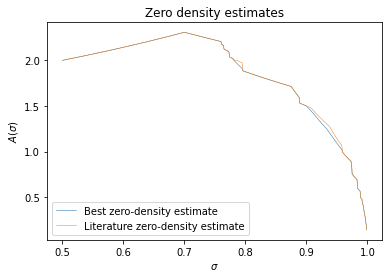
\includegraphics[width=0.5\linewidth]{chapter/zero_density_estimate_plot.png}
    \caption{The bounds in Table \ref{zero_density_estimates_table}, compared against the existing literature bounds on $\A(\sigma)$.}
    \label{fig:zero_density_estimate}
\end{figure}

For completeness, we list in Table \ref{zero_density_historical} some historical zero density theorems not already covered, which have now been superseded by more recent estimates.

\begin{table}[ht]
    \def\arraystretch{1.3}
    \centering
    \caption{Historical upper bounds on $\A(\sigma)$}
    \begin{tabular}{|c|c|c|}
    \hline
    $\A(\sigma)$ bound & Range & Reference\\
    \hline
    $4\sigma$ & $\frac{1}{2} \leq \sigma \le 1$ & Carlson (1921) \cite{carlson_uber_1921}\\
    \hline
    $2$ & $4/5 \leq \sigma \leq 1$ & Montgomery (1969) \cite{montgomery_1969} \\
    \hline
    $2$ & $0.8080 \leq \sigma \leq 1$ & Forti--Viola (1972) \cite{forti-viola} \\
    \hline
    $\frac{39}{115\sigma-75}$ & $55/67 \leq \sigma \leq 189/230$ & Huxley (1973) \cite{huxley_large_1973} \\
    \hline
    $2$ & $189/230 \leq \sigma \leq 78/89$ & Huxley (1973) \cite{huxley_large_1973} \\
    \hline
    $\frac{48}{37(2\sigma-1)}$ & $78/89 \leq \sigma \leq 61/74$ & Huxley (1973) \cite{huxley_large_1973} \\
    \hline
    $\frac{3}{2\sigma}$ & $37/42 \leq \sigma \leq 1$ & Huxley (1975) \cite{huxley_large_1975a}\\
    \hline
    $\frac{48}{37(2\sigma-1)}$ & $61/74 \leq \sigma \leq 37/42$ & Huxley (1975) \cite{huxley_large_1975a}\\
    \hline
    $2$ & $0.80119 \leq \sigma \leq 1$ & Huxley (1975) \cite{huxley_large_1975a}\\
    \hline
    $2$ & $4/5 \leq \sigma \leq 1$ & Huxley (1975) \cite{huxley_large_1975b}\\
    \hline
    $\frac{6}{5\sigma-1}$ & $67/87 \leq \sigma \leq 1$ & Ivi\'c (1979) \cite{ivic_note_1979} \\
    \hline
    $\frac{3}{34\sigma-25}$ & $28/37 \leq \sigma \leq 74/95$ & Ivi\'c (1979) \cite{ivic_note_1979} \\
    \hline
    $\frac{9}{7\sigma-1}$ & $74/95 \leq \sigma \leq 1$ & Ivi\'c (1979) \cite{ivic_note_1979} \\
    \hline
    $\frac{3}{2\sigma}$ & $4/5 \leq \sigma \leq 1$ & Ivi\'c (1979) \cite{ivic_note_1979} \\
    \hline
    $\frac{68}{98\sigma-47}$ & $115/166 \leq \sigma \leq 1$ & Ivi\'c (1979) \cite{ivic_note_1979} \\
    \hline
    $\frac{3}{2\sigma}$ & $3831/4791 \leq \sigma \leq 1$ & Ivi\'c (1980) \cite{ivic_exponent_pairs}  \\
    \hline
    $\frac{9}{7\sigma-1}$ & $41/53 \leq \sigma \leq 1$ & Ivi\'c (1980) \cite{ivic_exponent_pairs} \\
    \hline
    $\frac{6}{5\sigma-1}$ & $13/17 \leq \sigma \leq 1$ & Ivi\'c (1980) \cite{ivic_exponent_pairs} \\
    \hline
    $\frac{4}{2\sigma+1}$ & $17/18 \leq \sigma \leq 1$ & Ivi\'c (1980) \cite{ivic_exponent_pairs} \\
    \hline
    $\frac{24}{30\sigma-11}$ & $155/174 \leq \sigma \leq 17/18$ & Ivi\'c (1980) \cite{ivic_exponent_pairs} \\
    \hline
    $\frac{3}{7\sigma-4}$ & $3/4 \leq \sigma \leq 10/13$ & Ivi\'c (1983) \cite{ivic_topics_1983} \\
    \hline
    $\frac{9}{8\sigma-2}$ & $10/13 \leq \sigma \leq 1$ & Ivi\'c (1983) \cite{ivic_topics_1983} \\
    \hline
    $\frac{15}{22\sigma-10}$ & $10/13 \leq \sigma \leq 5/6$ & Ivi\'c (1984) \cite{ivic_zero_1984} \\
    \hline
    $\frac{3k}{(3k-2)\sigma+2-k}$ & $\frac{9k^2 -3k + 2}{12k^2 -5k + 2} \leq \sigma \leq 1$; $k \geq 2$ & Ivi\'c (1984) \cite{ivic_zero_1984} \\
    \hline
    $58.05 (1-\sigma)^{1/2}$ & $1/2 \leq \sigma \leq 1$ & Ford (2002) \cite{FordZeta} \\
    \hline
    $6.42 (1-\sigma)^{1/2}$ & $9/10 \leq \sigma \leq 1$ & Heath-Brown (2017) \cite{heathbrown_new_2017} \\
    \hline
    $3\sqrt{2}(1-\sigma)^{1/2}+18(1-\sigma)$ & $17/18 \leq \sigma \leq 1$ & Pintz (2023) \cite{pintz_density_2023}\\
    \hline
    \end{tabular}
    \label{zero_density_historical}
    \end{table}

{\bf TODO: enter this table into literature.py}

\section{Estimates for \texorpdfstring{$\sigma$}{sigma} very close to \texorpdfstring{$1/2$}{1/2} or \texorpdfstring{$1$}{1}}

Some additional estimates were established for $\sigma$ sufficiently close to $1/2$ or $1$.

Tur\'an \cite{turan} introduced the power sum method to establish
$$ \A(1-\eta) \leq 2 + \eta^{0.14}$$
for $\eta$ small enough. Hal\'asz and Tur\'an \cite{halasz_distribution_1969} combined this method with the large values approach of Hal\'asz \cite{halasz_1968} to improve the bound to
\begin{equation}\label{a-eta}
  \A(1-\eta) \leq C \eta^{1/2}
\end{equation}
with $C = 12,000$ for sufficiently small $\eta$.  See \cite{pintz_2022} for an alternate proof of these results.

The constant $C$ in \eqref{a-eta} was improved to $1304.37$ by Montgomery \cite[Theorem 12.3]{montgomery_topics_1971} (see also the remark after \cite[(11.97)]{ivic} for a correction), to $58.05$ by Ford \cite{FordZeta}, to $5.03$ by Heath-Brown \cite{heathbrown_new_2017} (the latter exploiting the resolution of the Vinogradov mean value conjecture \cite{bourgain_demeter_guth}), and to any $C > 3\sqrt{2}=4.242\dots$ in \cite{pintz_density_2023}. See also an explicit version at \cite{bellotti}.

``Log-free'' zero density estimates of the form
$$ N(1-\eta,T) \ll T^{B\eta}$$
for various $B$ were established starting with the work of Linnik \cite{linnik-1,linnik-2} and developed further in \cite{turan}, \cite{fogels}, \cite{bombieri_1974}, \cite{jutila_linnik}, \cite{gallagher_large_sieve}, \cite{graham_1978}, \cite{heath_brown_least_prime}. An explicit version of such estimates may be found in \cite{bellotti_2024}.

There is some work establishing bounds on $N(\sigma,T)$ for $\sigma$ very close to $1/2$ (and not necessarily fixed), although these bounds do not make further improvements on $\A(\sigma)$.  Specifically, bounds of the form
$$ N(\sigma,T) \ll T^{1-\theta(2\sigma-1)} \log T$$
for $T \geq 2$ (say) were established for $\theta=1/8$ by Selberg \cite{selberg_1946} (see \cite{simonic} for an explicit version), any $0 < \theta < 1/2$ by Jutila \cite{jutila-critical}, and any $0 < \theta < 4/7$ by Conrey (claimed in \cite{conrey_at_1989}, with a full proof given in \cite{baluyot_thesis}).  Note that the density hypothesis would follow if we could establish the claim for all $0 < \theta < 1$, but an improvement to Ingham's bound (Theorem \ref{thm:ingham_zero_density2}) would only occur once $\theta$ exceeded $2/3$.

\section{A heuristic for zero density estimates}

We can now state a rough heuristic as to what zero density estimates to expect from a given large value theorem:

\begin{heuristic}[Predicting a zero density estimate from a large value theorem]\label{lv-heuristic}\uses{lv-def, zero-def} Suppose that $1/2 \leq \sigma \leq 1$ and $\tau_0 \geq 1$ are such that one can prove $\LV(\sigma, \tau_0) \leq 3-3\sigma$ (i.e., the Montgomery conjecture holds here with a multiplicative loss of $3/2$).  Then in principle, one can hope to prove $\A(\sigma) \leq 3/\tau_0$.  Conversely, if one cannot prove $\LV(\sigma, \tau_0) \leq 3-3\sigma$, then the bound $\A(\sigma) \leq 3/\tau_0$ is likely out of reach.
\end{heuristic}

We justify this heuristic as follows, though we stress that the arguments that follow are not fully rigorous.  In the first part, we simply apply Corollary \ref{zero-large-cor2}.  In practice, the \eqref{lvo} is often more delicate than \eqref{lvoz} and ends up being the limiting factor for the bounds; furthermore, within \eqref{lvo}, it is the right endpoint $\tau=\tau_0$ of the range $2\tau_0/3 \leq \tau \leq \tau_0$ that ends up being the bottleneck; but this is precisely the claimed criterion $\LV(\sigma, \tau_0) \leq 3-3\sigma$.  We remark that in some cases (particularly for $\sigma$ close to one), the estimate \eqref{lvoz} ends up being more of the bottleneck than \eqref{lvo}, and so one should view $3/\tau_0$ here as a theoretical upper limit of methods rather than as a guaranteed bound.  (In particular, the need to also establish the bound $\LV_\zeta(\sigma, \frac{4}{3}\tau_0-\eps) < 4-4\sigma$ for $\eps>0$ small can sometimes be a more limiting factor.)

Conversely, suppose that
\begin{equation}\label{lst3}
    \LV(\sigma,\tau_0) > 3-3\sigma,
\end{equation}
but that one still wants to prove the bound $\A(\sigma) \leq 3/\tau_0$. Heuristically, Theorem \ref{zero-dens_implies_large} suggests that in order to do this, it is necessary to establish the bound $\LV_\zeta(\sigma,\tau)/\tau \leq \frac{3}{\tau_0}(1-\sigma)$ for all $\tau \geq 2$.  In particular, one should show that
$$ \LV_\zeta(\sigma,2\tau_0) \leq 6-6\sigma.$$
Let us consider the various options one has to do this.  There are ways to control zeta large values that do not apply to general large value estimates, such as moment estimates of the zeta function, exponent pairs, or control of $\beta$ and $\mu$.  However, at our current level of understanding, these techniques only control $\LV_\zeta(\sigma,\tau)$ for relatively small values of $\tau$, and in practice $2\tau_0$ is too large for these methods to apply; this exponent also tends to be too large for direct application of standard large value theorems to be useful.  Hence, the most viable option in practice is raising to a power (Lemma \ref{power-lemma}), using
$$ \LV_\zeta(\sigma,2\tau_0) \leq k \LV_\zeta(\sigma,2\tau_0/k)$$
for some natural number $k \geq 2$.  However, the most natural choice $k=2$ is blocked due to our hypothesis \eqref{lst3}, while in practice the $k \geq 3$ choice is blocked because of Lemma \ref{lv-lower}.  Hence it appears heuristically quite difficult to establish $\A(\sigma) \leq 3/\tau_0$ with current technology, in the event that \eqref{lst3} occurs.

In Table \ref{zero_density_heuristic} we list some examples in which the heuristic can actually be attained.  Note that this only covers some, but not all, of the best known zero density estimates in Table \ref{zero_density_estimates_table}, as there are often other bounds that need to be established that prevent the heuristic limit of $3/\tau_0$ from actually being attained; so one should take the heuristic with a certain grain of salt.

\begin{table}[ht]
    \def\arraystretch{1.3}
    \centering
    \caption{Examples of large value theorems, the values of $\tau_0$ and $\A(\sigma)$ they suggest, and rigorous zero density theorems that attain the predicted value for at least some ranges of $\sigma$.}
    \begin{tabular}{|c|c|c|c|}
    \hline
    Large value theorem & Predicted choice of $\tau_0$ & Predicted bound $\frac{3}{\tau_0}$ on $\A(\sigma)$ & Matching zero density theorem(s)\\
    \hline
    Theorem \ref{l2-mvt} & $2-\sigma$ & $\frac{3}{2-\sigma}$ & Theorem \ref{thm:ingham_zero_density2}\\
    \hline
    Theorem \ref{huxley-lv} & $3\sigma-1$ & $\frac{3}{3\sigma-1}$ & Theorem \ref{huxley-bound} \\
    \hline
    Theorem \ref{hb-opt} & $10\sigma-7$ & $\frac{3}{10\sigma-7}$ & Theorems \ref{hb-density}, \ref{hb-density2} \\
    \hline
    Theorem \ref{jutila-lvt}, $k=3$ & $\frac{7\sigma-1}{3}$ & $\frac{9}{7\sigma-1}$ & Theorems \ref{hb-density}, \ref{further_ivic_zero} \\
    \hline
    Lemma \ref{a-ivt-1}, $m=2$ & $\frac{4\sigma}{2}$ & $\frac{3}{2\sigma}$ & Corollary \ref{further_ivic_zero}, Theorem \ref{bourgain-zero-density-2000} \\
    \hline
    Lemma \ref{a-ivt-1}, $m=3$ & $\frac{7\sigma-1}{3}$ & $\frac{9}{7\sigma-1}$ & Theorems \ref{hb-density}, Corollary \ref{further_ivic_zero} \\
    \hline
    Lemma \ref{a-ivt-1}, $m=4$ & $\frac{10\sigma-2}{4}$ & $\frac{6}{5\sigma-1}$ & Corollary \ref{further_ivic_zero} \\
    \hline
    Lemma \ref{a-ivt} & $7\sigma-4$ & $\frac{3}{7\sigma-4}$ & Corollary \ref{ivic-near-34} \\
    \hline
    Lemma \ref{a-ivt} & $\frac{8\sigma-2}{3}$ & $\frac{9}{8\sigma-2}$ & Corollary \ref{ivic-near-34} \\
    \hline
    Theorem \ref{guth-maynard-lvt} & $\frac{5\sigma-3}{3}$ & $\frac{15}{5\sigma-3}$ & Theorem \ref{guth-maynard-density} \\
    \hline
    \end{tabular}
    \label{zero_density_heuristic}
    \end{table}

    One consequence of Heuristic \ref{lv-heuristic} is that, in the regimes where the heuristic is accurate, combining multiple large values theorems together are unlikely to achieve new zero density theorems that could not be accomplished with each large value theorem separately.
    
\section{Explicit results}
A number of explicit versions of the above zero-density estimates have been established, which are particularly relevant when $\sigma$ is close to $1/2$ or $1$, where factors of $T^{o(1)}$ become significant. 

\begin{theorem}[\cite{simonic}]
For $T \ge 3$ and $1/2 \le \sigma \le 0.778$, one has
$$
N(\sigma, 2 T)-N(\sigma, T) \leq  5874.051 T^{1-\frac{1}{4}\left(\sigma-\frac{1}{2}\right)} \log T+ 1.107 \log ^2 T + 0.345\log T \log \log T.
$$
\end{theorem}
Sharper bounds for $T$ large can be found in \cite{simonic}.

\begin{theorem}[\cite{chourasiya_explicit_2025}]For every $T\ge 3 $ and $1/2\le \sigma\le 5/8$ one has
\[
N(\sigma, T) \leq 8.604 T^{\frac{3(1-\sigma)}{2-\sigma}} \log ^3 T+9.461 \log ^2 T+167.8 \log T.
\]
For every $T\ge 3 $ and $5/8\le \sigma\le 7/8$ one has
    \[
    N(\sigma, T) \leq 22.44 T^{\frac{3(1-\sigma)}{2-\sigma}} \log ^3 T+8.290 \log ^2 T+147.0 \log T.
    \]
\end{theorem}

\begin{theorem}[\cite{chourasiya_explicit_2024}]For every $T\ge 3$ and $\sigma\ge 3/5$, one has
    \begin{equation*}
N(\sigma, T) \leq 0.7756 T^{4 \sigma(1-\sigma)} \log ^{5-2 \sigma} T.
\end{equation*}
\end{theorem}
Further bounds for larger values of $\sigma$ can be found in \cite{chourasiya_explicit_2024}.

\begin{theorem}[\cite{ramare_explicit_2016}]\label{th:ramareexpl} For every $T\ge 3$ and $\sigma\ge 0.52$ one has
    \begin{equation*}
N(\sigma, T) \leq 965(3 T)^{\frac{8(1-\sigma)}{3}}(\log T)^{5-2 \sigma}+51.5(\log T)^2.
\end{equation*}
\end{theorem}

The following result is an improvement upon \cref{th:ramareexpl}.
\begin{theorem}[\cite{Kadiri_explicit_2018}]\label{th:explicitkln}
For each tuple ($\sigma_0, A, B)$ of Table \ref{zerodensity_kadiri}, one has
\[
N(\sigma, T) \leq AT^{\frac{8}{3}(1-\sigma)}(\log T)^{5-2\sigma} + B(\log T)^2
\]
for each $\sigma_0 \le \sigma \le 1$ and $T \ge 3$.
\end{theorem}

\begin{table}[ht]
\centering
\begin{tabular}{|c|c|c|}
\hline
$\sigma_0$ & $A$ & $B$ \\
\hline
0.75 & 5.277 & 4.403 \\
0.80 & 6.918 & 3.997 \\
0.85 & 8.975 & 3.588 \\
0.90 & 11.499 & 3.186 \\
0.95 & 14.513 & 2.772 \\
0.98 & 16.544 & 2.532 \\
\hline
\end{tabular}
\caption{Some examples of ($\sigma_0, A, B)$}
\label{zerodensity_kadiri}
\end{table}
See \cite{Kadiri_explicit_2018} for further estimates.\\
The following result is an explicit log-free zero density estimate.
\begin{theorem}[\cite{bellotti_2024}]\label{th:explbellogfree}
For every $T\ge 3$ and $\sigma\in[0.9927,1]$, one has $$N(\sigma, T) \leq 4.45 \cdot 10^{12} \cdot T^{8(1-\sigma)}.$$
\end{theorem}
Sharper estimates of the form
$$N(\sigma,T)\le CT^{B(1-\sigma)},\qquad \sigma\in[\sigma_0,1],\quad T\in[T_0,T_1]$$ can be found in \cite{bellotti_2024}. We mention a couple of examples in Table \ref{table:bellottilogfree}.
\begin{table}[h]
\def\arraystretch{1.3}
\centering
\caption{Values of constants $C,B$}
\begin{tabular}{|c|c|c|c|c|}
\hline
 $B$ & $C$ & $\sigma_0$ & $T_0$ & $T_1$ \\
\hline
$1.551$ & $1.62\cdot 10^{11}$ & $0.9927$ & $3$ & $\exp(6.7\cdot 10^{12})$\\
\hline
$1.551$ & $1.62\cdot 10^{11}$ & $0.985$ & $\exp(80)$ & $\exp(6.7\cdot 10^{12})$\\
\hline
\end{tabular}
\label{table:bellottilogfree}
\end{table}
\begin{theorem}[\cite{bellotti}]\label{th:explicitkvbel}
For every $\sigma\in[0.98,1]$ and $T\ge 3$, one has:\begin{equation*}
    N(\sigma,T)\le2.15\cdot 10^{23}\cdot T^{57.8875(1-\sigma)^{3/2}}(\log T)^{10393/900}.
\end{equation*}
\end{theorem}
Note that \cref{th:explicitkvbel} implies the following log-free zero-density bound.
\begin{corollary}[\cite{bellotti_2024}]\label{th:kvaslokgfreebel}
For every $T\ge \exp(6.7\cdot 10^{12})$ and $\sigma\in[0.98,1]$, one has$$N(\sigma, T) \leq 4.45 \cdot 10^{12} \cdot T^{11.3(1-\sigma)}.$$
\end{corollary}



